\documentclass[utf8]{ctexart}
\author{syx}

\usepackage{graphicx}
\usepackage{ulem}
\usepackage{microtype}
\usepackage{geometry}
\usepackage{exscale}
\usepackage{relsize}

\geometry{left=3.5cm,right=3.5cm,top=4cm,bottom=4cm}

\begin{document}
	\section*{寒假作业}
	\subsection*{题目:}
	研究带缺口圆环的逾渗模型及其电导率。
	\subsection*{算法:}
	本题思路为,先在二维正方形格点中画出图形,再利用普通的座逾渗模型计算逾渗阈值$p_c$。

	首先是在格点上画出圆形。建立二维数组A[N][N]表示格点,矩阵元$a_{ij}$存储该点是否被占据的信息,数组下标$i,j$代表将二维数组置于平面格点上时每点的坐标。
	画出圆形,只需在一定范围内遍历网格,判断当前格点是否满足约束约束$R_1\leq\sqrt{i^2+j^2}\leq R_2$。

	画出缺口则略微复杂。我们设圆形缺口的对称轴与$x$轴夹角为$\theta$,每次需计算当前格点到圆心的连线与$x$轴的角度,算出两个角度对应的角度差$\phi$,判断是否小于缺口张角的一半从而决定是否画出即可。程序中使用atan2()函数将直线斜率转换为角度大小。
	画第$n$个圆时,在圆对应的所有格点上标记数字$n$。为了在每点存储多于一个数字,程序中使用
	二维可变长向量数组,每个矩阵元都为一个可变长向量。画出$n$个圆的时间显然是$O(n)$的。

	其次是判断上下是否连通。本题认为若两个点上下或左右相邻,则属于同一集团。首先将上边界设为集合\{1\},下边界设为集合\{2\}。对每个格点,收集它以及它相邻格点包含的数字,组成新的集合,并将所有集合都存入一维向量中。之后判断该集合中的数字是否出现在先前的集合中,如果出现了,则说明该点与先前集合中的点是连通的,将其合并为一个大集合;如果未出现,则说明该集合中的点独立于之前的点,不进行操作。每次从第二个集合开始直到最后一个集合,判断其是否属于之前的集合,直到某一整次判断中,没有任何集合被合并。如果1,2在一个集合中,则说明上下边界连通,否则不连通。此方法总时间是$O(n^2)$的。

	最后是计算电导率,利用了电导率矩阵方法,参考Derrida的strip法(如下图)。\\
	\includegraphics[width=0.66\textwidth]{shot1.png}\\
	
	我们将相邻的两个格点等效为图中的电阻器,且阻值较低,其他位置等效为高阻值电阻器。
	图中的每个$I$都依赖于$U$,即$I_i=\sum_{j}\sigma_{ij}U_j$。此方法需要从左至右计算每个电阻加入网络后对电导矩阵$\sigma_{ij}$的作用,不断更新电导矩阵,最后根据$\frac{\mathrm{d}I_1}{\mathrm{d}U_1}=\sigma_{11}$得到整体电导,在此不再详细介绍。由于每次操作需要改变整个矩阵,操作次数取决于点的个数,因此此过程的时间是$O(n^4)$的,是程序的主要耗时部分。

	绘图时,直接将每个格点的占据状态对应为一个像素信息即可。为了更加直观的看到连通状况,图中红色部分表示与上边界联通的占据点,蓝色表示与下边界连通的占据点,若上下连通,则全为红色。其余部分白色表示未占据点,深色表示未连接至大集团的孤立集团。
	
	\subsection*{数据:}
	\noindent
	下图为低于逾渗阈值的状态,集团规模较小,上下明显无法导通$(p_c=0.0716)$:\\
	\includegraphics[width=\textwidth]{img_4_1.png}\\
	\clearpage
	下图为逾渗阈值附近的状态,大集团的规模开始增大$(p_c=0.0748)$:\\
	\includegraphics[width=\textwidth]{img_6_2.png}\\
	\clearpage
	概率不变,出现了接近导通的临界状态$(p_c=0.0748)$:\\
	\includegraphics[width=\textwidth]{img_6_1.png}\\
	\clearpage
	高于逾渗阈值,已经完全导通$(p_c=0.0793)$:\\
	\includegraphics[width=\textwidth]{img_8_2.png}\\
	\clearpage
	\noindent 以上数据为$10240\times10240$的格点,每个圆环内径100,外径103.5。
	对应的逾渗概率结果为:\\
	\includegraphics[width=\textwidth]{fig1.jpg}\\
	为了快速迭代,我们缩小格点的数量,大量模拟来求出占据概率与逾渗概率的关系。\\
	下图为$2048\times2048$,内径30,外径31.5的结果。
	以下每个概率求20组,将结果画出:\\
	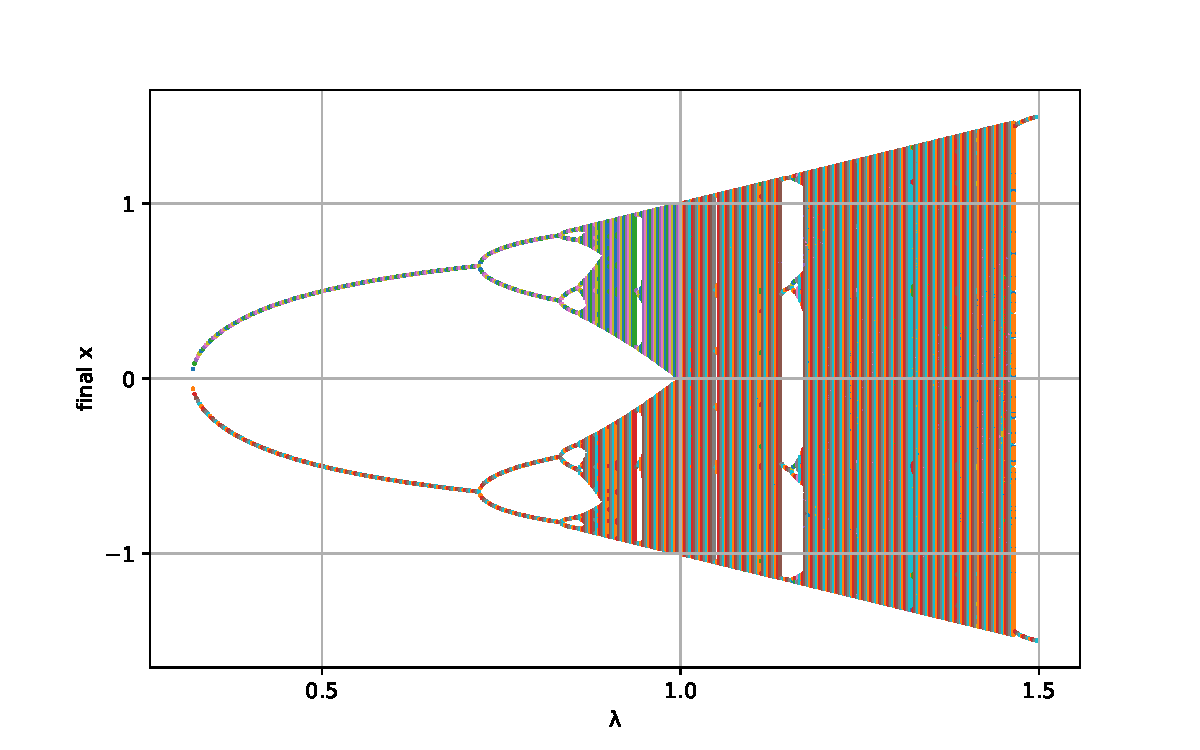
\includegraphics[width=\textwidth]{fig2.jpg}\\
	从图中可以发现,该模型的逾渗阈值约为$p_c=0.082$

	最后是电导率。由于该算法费时较多,我们进一步缩小点阵大小$(400\times400,20,21.5)$,结果如下图:\\
	\includegraphics[width=0.4\textwidth]{img_2_1.png}
	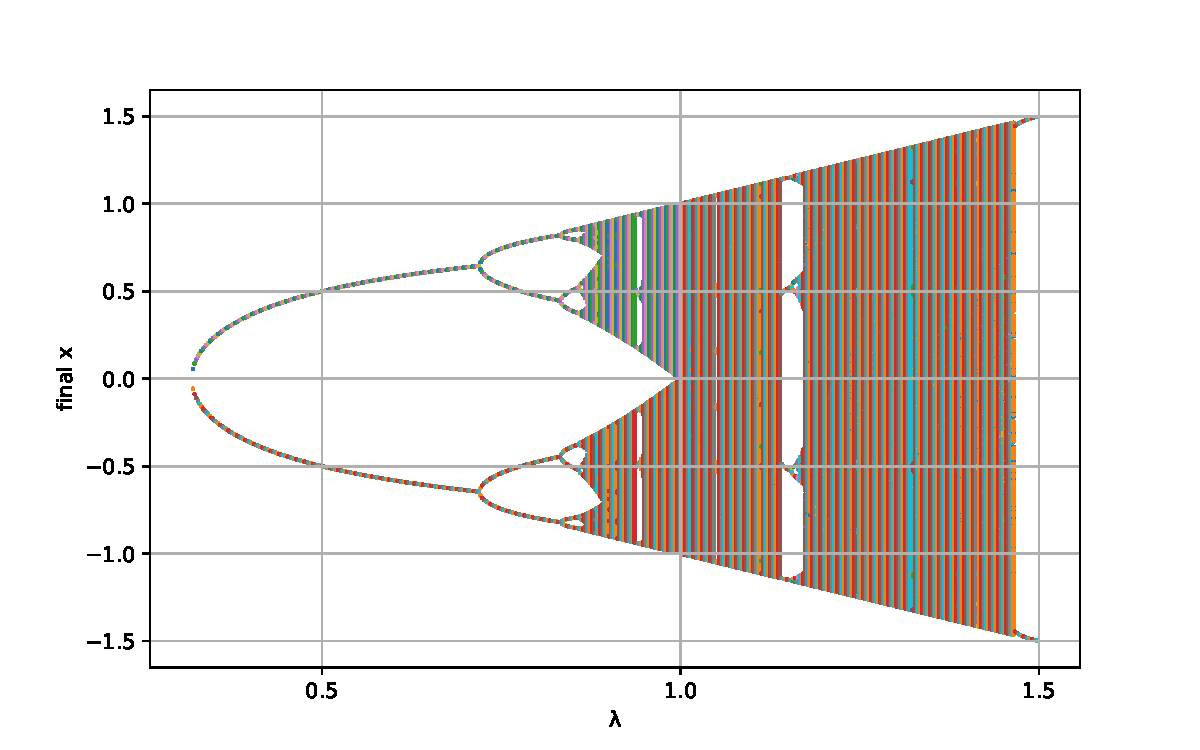
\includegraphics[width=0.6\textwidth]{fig3.jpg}
	多次计算,得到电导率变化为:\\
	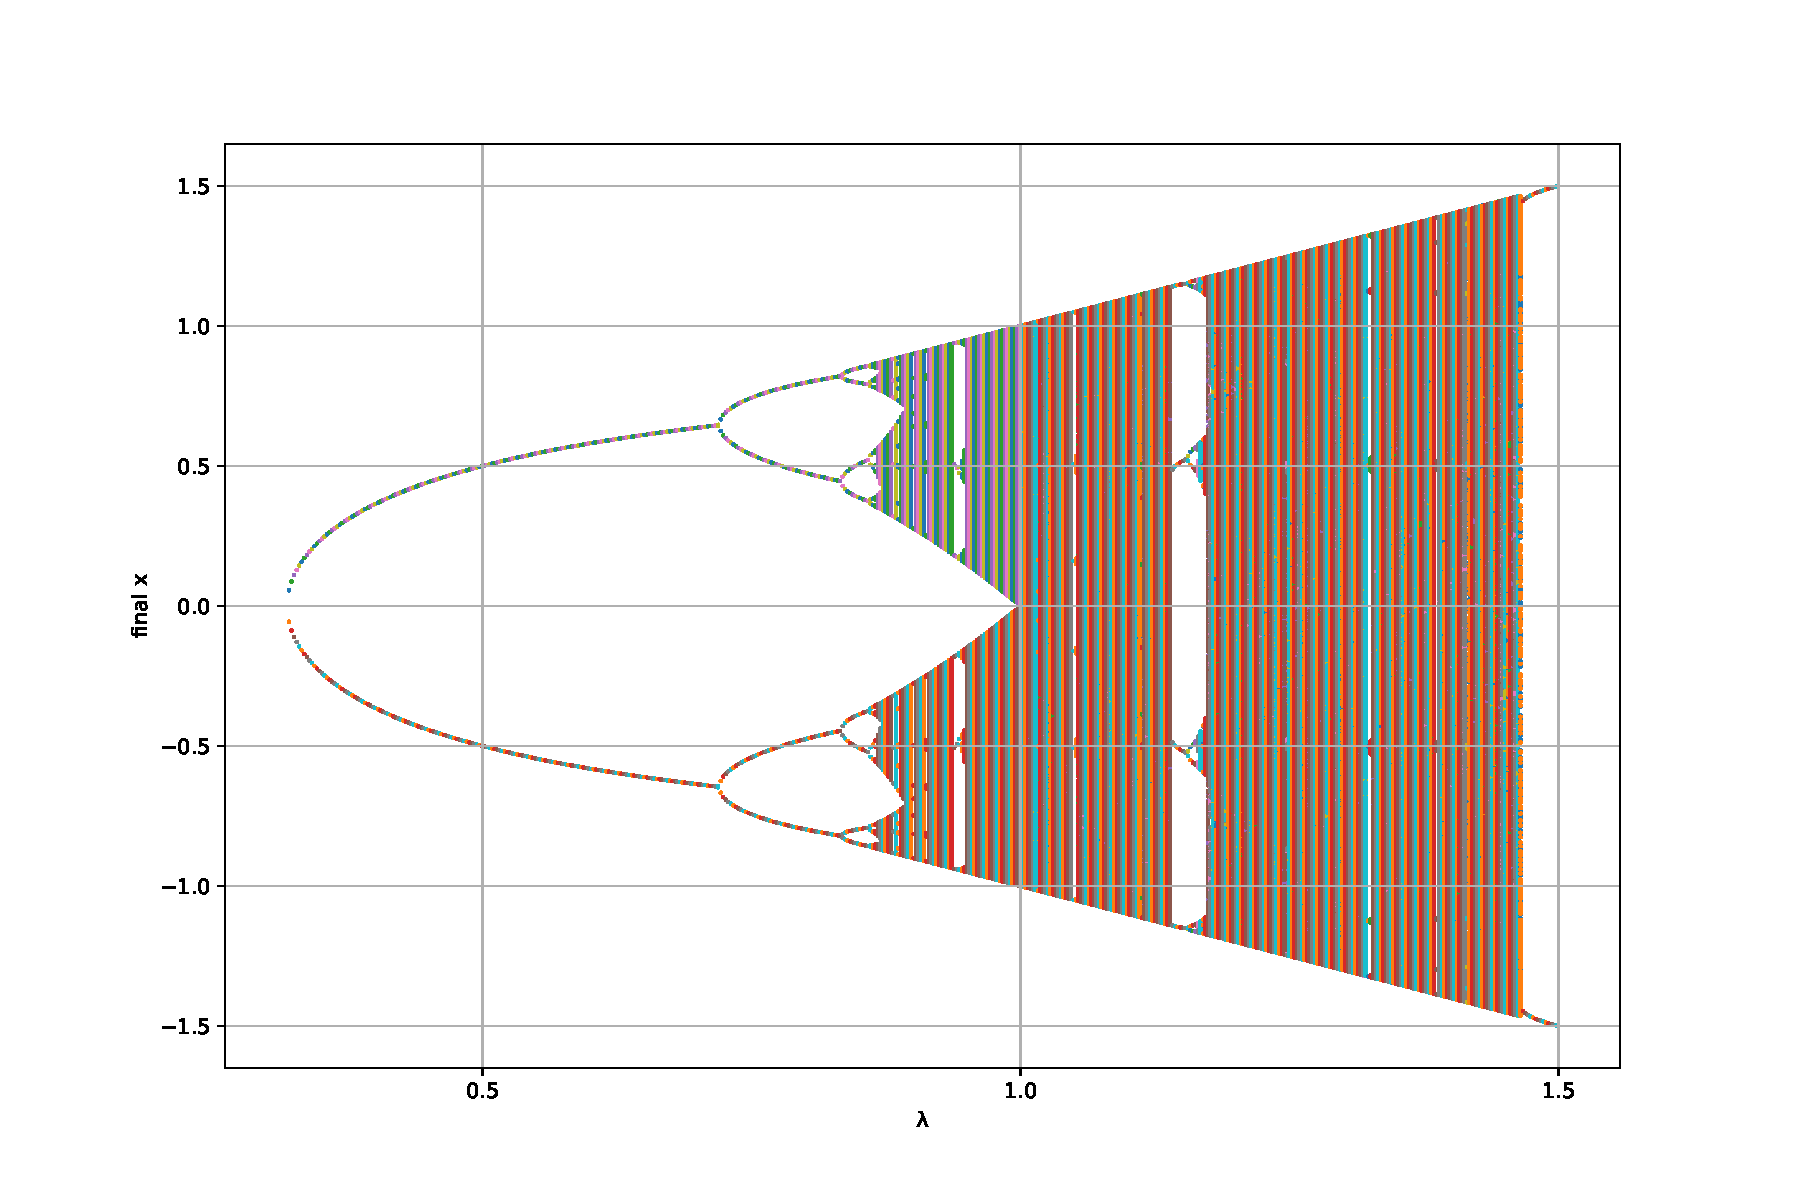
\includegraphics[width=\textwidth]{fig4.jpg}\\

	\subsection*{讨论:}
	从以上模拟结果中,我们可以得出逾渗阈值的范围大约在$0.0748\sim0.0995$之间,且基本不随我们观察的尺度变化。相对于逾渗概率,电导率的变化更加平滑,对应一级相变与二级相变的区别。

	在模拟中,我们更换了不同的网格大小,实际上对结果没有特别大的影响。如果我们的模型不是格点模型而是连续逾渗模型,那么尺度变化对我们模拟的结果将没有任何影响:设想将我们模拟的结果线度缩小一半,在缩小前后,图形是相似的,因此所有的物理量都不改变;这时,用4个缩小后的图形拼接为原大小的图形,所得图形的逾渗阈值、电导率(不具有长度量纲)都不会变化,但其中的圆环大小发生了改变。因此只要保证圆环的形状不变,理论上逾渗的性质就不会改变。在实际模拟中,缩小模拟的尺度时,由于格点大小保持不变,所以画出的圆形状会有所变化,从而影响逾渗概率。当网格缩小时,圆形一起缩小,但圆环的半径差至少为1,这可能会造成圆环与以前相比更“粗”了,因此圆环数量不变时,逾渗阈值(即占据点的比例)略有增加。另外,用有限大小的网格模拟,不同的尺度下边界效应不同,也会影响到结果。

	实验的不足之处在于算法性能不够好,需要大量的时间来计算,因此数据点数量略有不足。获得了足够多的数据点后,才能拟合出准确的曲线,探究逾渗阈值附近相变指数的大小。
	
	
\end{document}